\section{Analysis}
\label{sec:analysis}

\subsection{Data Exploration}
\label{subsec:data_exploration}
From the \textit{Yahoo Finance} website some features can be achieved from each stock company. It is provided the same features to every company listed.
These are the features:\\
\begin{itemize}
  \item \textbf{Open Price:}
    Is defined as the price of the first trade of the day. It is common that the opening price is not identical
    to the last closing price. This occurs as effect of the investors' expectations outside the trading hours.\\
  \item \textbf{High price} and \textbf{Low price:}
    The high price is defined as the highest price at which a stock traded over the day, while the low price is the lowest price. Analyzing these values it is
    possible to find gaps or sudden jumps in a stock's price when there was not trading between those two prices.\\ 
  \item \textbf{Volume:} 
    Is defined as the number of transactions occurred in a day. The volume is an important measure of strength of the prices. If the volume is 
    higher than average, it is a sign that a particular stock price is getting stronger. Therefore, analyzing the volume high helps to understand the price
    movement.\\

  \item \textbf{Close Price:}
    Is defined as the price of the last trade of the day. Although it does not mandatorily reflect the next's day opening price, this value is
    important for investors to analyze changes in stock prices over time. Comparing closing prices, investors can measure the market sentiment over a period.\\
 
  \item \textbf{Adjustment Closing Price:}
    Is defined as a stock's closing price that has been amended to include all corporate actions, such as stock splits, dividends/distributions and right offerings, that
    occurred at any time before the next's day opening price. This marker gives analysts an accurate representation of the company's equity value beyond the simple market price.
    This feature is often used to study the company's historical performance.\\

\end{itemize} 
\ \\
To develop this project one company needed to be chosen. In order to understand better all the data available, and study the best algorithms, some points about a company were defined: The
company should be on the market for the least five years and, in this period, demonstrated some soft price variation.
This condition was based on the objective of this project: It will not to determine when some company will break or rise. It will only predict for some period if the company stocks will
be valorized or not. In order to determine the sentiment of a company to predict if it will break or not, would be necessary data from other sources, such as twitter.
However, this project will remain as an open source code and eventually will be developed to work with new features. 
Therefore, considering all the points stated before, the company \textbf{NVS - Norvatis AG Common Stock}  was chosen and the following results will be from it.\\


\subsection{Exploratory Visualization}
\label{subsec:Exploratory_visu}
The first step is to understand the dependency between the features. Plotting the correlation between the data, the following images were generated:\\

\begin{figure}[H]
\centering
\begin{subfigure}{.5\textwidth}
  \centering
  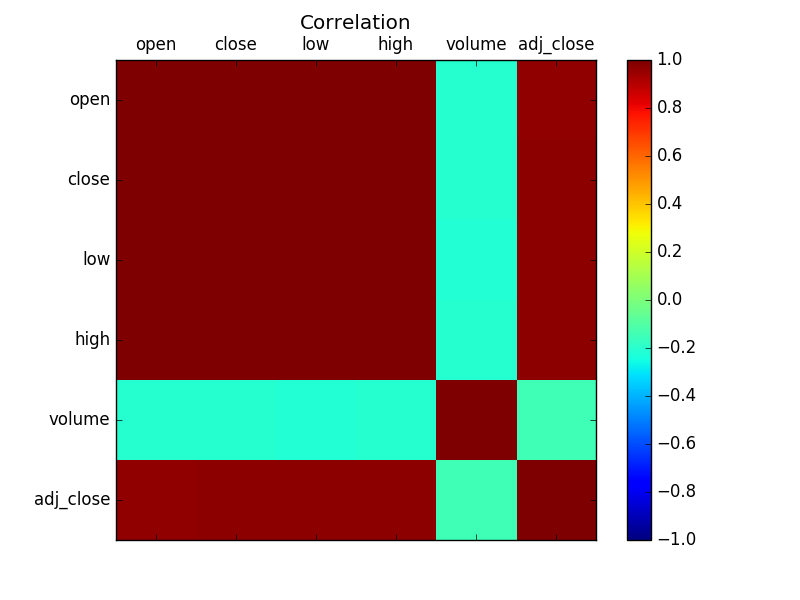
\includegraphics[width=.8\linewidth]{figures/correlation_nvs.png}
  \caption{Correlation graphic}
  \label{fig:nvs_correlation}
\end{subfigure}%
\begin{subfigure}{.5\textwidth}
  \centering
  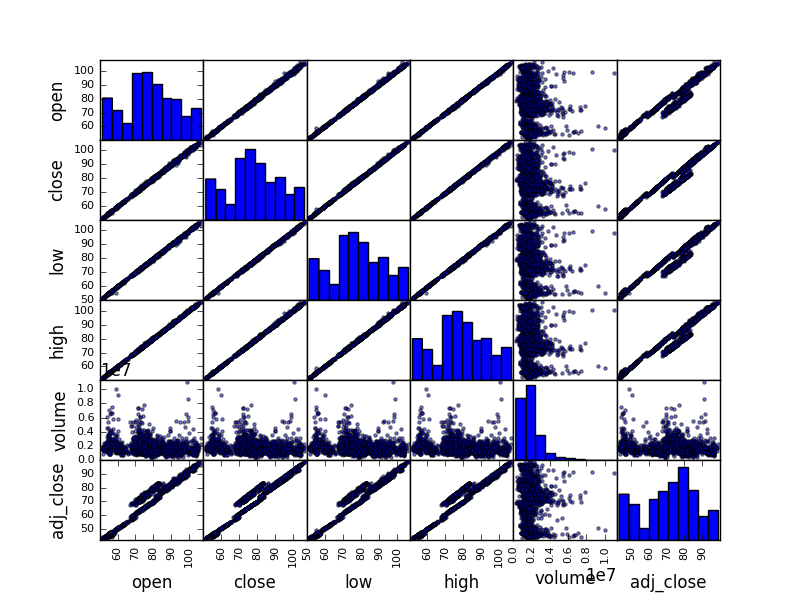
\includegraphics[width=.8\linewidth]{figures/scatter_matrix_nvs.png}
  \caption{Scatter matrix graphic}
  \label{fig:nvs_scatter_matrix}
\end{subfigure}
\caption{Correlation between features of the dataset}
\label{fig:features_correlation}
\end{figure}
\ \\
Analyzing the Figure \ref{fig:nvs_correlation} and the Figure \ref{fig:nvs_scatter_matrix}, it is clear that all the features, except to the Volume, are all correlated. For this project,
this means that can be used just one of them to build the model. The Volume feature does not seems to help with the model, so this feature will be excluded.
In the Figure \ref{fig:nvs_stock_results} three features are plot together, in order to understand their correlation.
\begin{figure}[H]
\centering
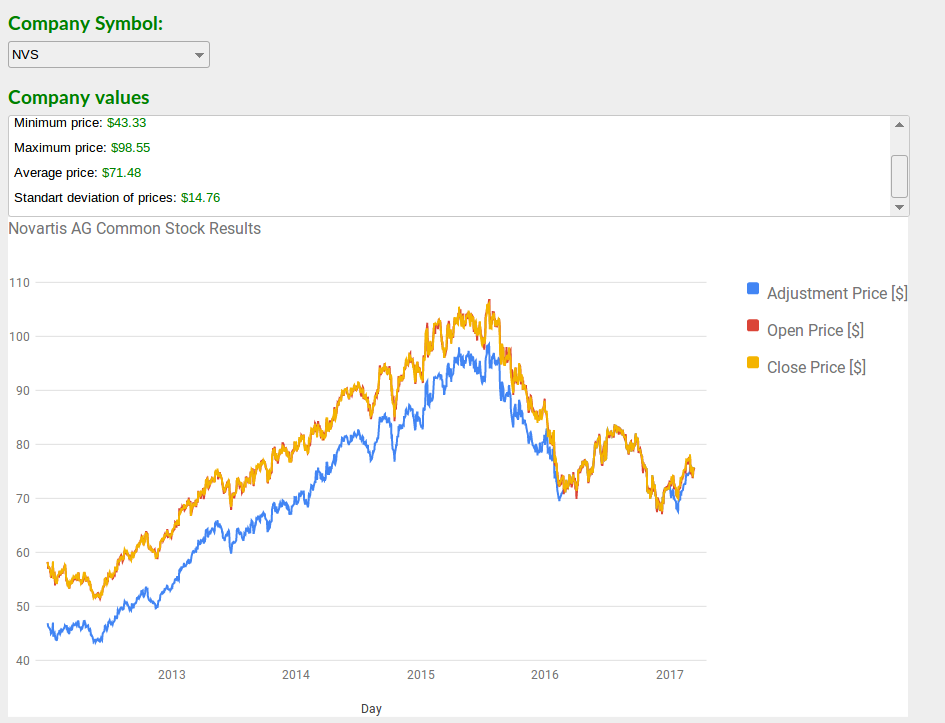
\includegraphics[width=0.8\textwidth]{figures/nvs_stock_results2.png}
\caption{\label{fig:data}For the past five years, the features Open, Close and Adjustment Price are displayed.}
\label{fig:nvs_stock_results}
\end{figure}

\subsection{Algorithms and Techniques}
\label{subsec:algorithm}
The result that this algorithm will predict is continous. This is a carctheristic of a linear problem, therefore, regression algorithms will be used to develop this model.
However, there are few different methods for linear regression. In order to choose one to work with, the following \textit{map} can be analyzed, represented on Figure \ref{fig:regression_map}.\\
\begin{figure}[H]
\centering
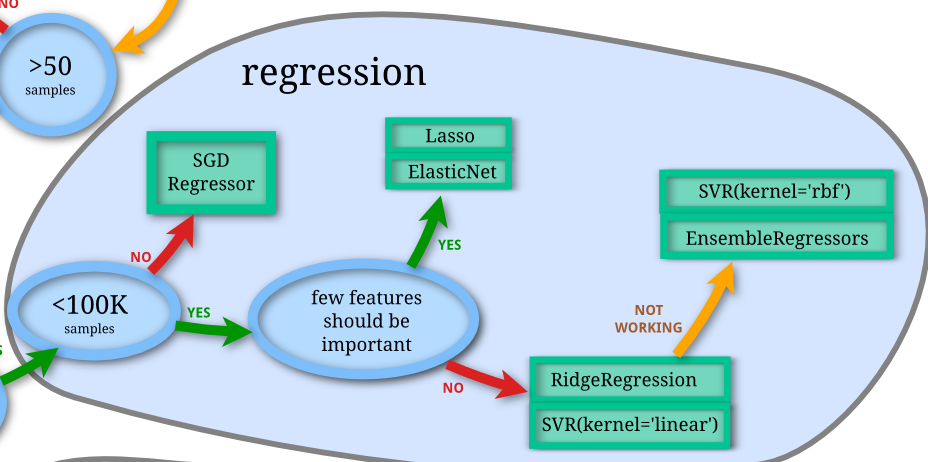
\includegraphics[width=0.8\textwidth]{figures/regression_map.png}
\caption{\label{fig:data} Scikit-learn algorithm cheat-sheet for regression.}
\label{fig:regression_map}
\end{figure}
\ \\
The dataset available is relatively small, it is smaller than one hundred thousand samples. The number of features are small, there is only six features available. The data that this 
algorithm will work also can not be defined as regression threes, since new data will be predicted - the next stock prices week.
The behavior of the data can not be estimated with a simple line or polynomial model. And, after analyzing all these points, the model selected to be used is the \textbf{Support Vector Machine - 
Support Vector Regressor}.\\
\\
The \textit{Support Vector Regression} algorithm is a good fit, because of the kernel trick. As others regression models, the \textit{SVR} present a method where it always try to fit a line
in between the points, and this line is designed to be always as far from the points as possible. But, this model also presents kernel options. Kernel is essentially a mapping function, which is
used to transform a given space in some other. There are few default kernel options available for SVR: Linear, Polynomial, RBF, Sigmoid, Precomputed or custom. And the one that fits better
this project is the RBF - Radio Basis Function Kernel. Also, the \textit{SVR} algorithm presents some others tune options. Once the model is defined, the easiest way to defined the best options
is to try each one and define which combination is better. There are a few tools available to perform it, consuming more cores of the processor, GPU, less RAM, and so on. It was implemented
the \textit{Pipeline} method, consuming 4 cores. The \textit{pipeline} is used to assemble several steps that can be cross-validated together setting different parameters.



\subsection{Benchmark}
\label{subsec:bench}
The result can be easily evaluated, since it will be quantifiable and compared to the already existing value. Therefore, the evaluation of the success of the model can be done by comparing the final
predicted value of the \emph{Adjusted Stock price} with the real one. The benchmark value, considering the $R^2 score$ (section \ref{sec:metrics}) for this project, that will be pursed initially will be of 0.5.
However, a value of 0.5 to predict stock prices does not seems to be reliable, since you cannot evaluate if the value of the stock is rising or decreasing over a period. 
Therefore, a reliable benchmark value to achieve when finishing this project would be around 0.9. With this value, the client using this software can interpret the values and decide if it is
a good scenario or not to keep/buy/sell stocks from this company.
\\